\documentclass{article}

\usepackage[utf8x]{inputenc}
\usepackage[english]{babel}
\usepackage[T1]{fontenc}
\usepackage{lmodern}
\usepackage{fullpage}
\usepackage{epstopdf}
\usepackage{graphicx}
\graphicspath{{../Images/}}
\usepackage{caption}
\usepackage{subcaption}
\usepackage{multirow}

% draw circuits
\usepackage{tikz}

% Math symbols
\usepackage{amsmath}
\usepackage{amssymb}
\usepackage{amsthm}

% Numbers and units
\usepackage{siunitx}

\usepackage[usenames,dvipsnames]{color}

\usepackage{todonotes}

\usepackage{hyperref}

\usepackage{listings}
\definecolor{gray}{rgb}{0.4,0.4,0.4}
\definecolor{dkgreen}{rgb}{0.25,0.7,0.35}
\definecolor{dkred}{rgb}{0.7,0,0} 
\lstset{language=matlab,numbers=left,numberstyle=\tiny\color{gray},basicstyle=\rm\footnotesize,keywordstyle=\bfseries\color{dkred},frame=single,commentstyle=\color{gray}=small, stringstyle=\color{dkgreen}}
% Matlab import
\usepackage{xparse}% for using parameters at the end block
\NewDocumentEnvironment{mylist}{m}{%
  \begin{#1}%
  % other code
}{%
  \end{#1}%
}

\NewDocumentEnvironment{mytable}{mm}
{\begin{table}[!ht]\centering}
{\caption{#2 Valeurs obtenues par le code du listing~\ref{lst:#1}.}\label{tab:#1}\end{table}}

\NewDocumentEnvironment{myfig}{mm}
{\begin{figure}[!ht]\centering}
{\caption{#2}\label{fig:#1}\end{figure}}
\NewDocumentEnvironment{myfigsub}{mmm}
{\begin{subfigure}[b]{#3\textwidth}}
{\caption{#2}\label{fig:#1}\end{subfigure}}

\newcommand{\mysubfig}[3]
{\begin{myfigsub}{#1}{#2}{#3}
    \includegraphics[width=\textwidth]{#1.png}
\end{myfigsub}}
\newcommand{\mysubfigg}[4]
{\begin{myfigsub}{#1}{#2}{#3}
    \includegraphics[#4, width=\textwidth]{#1.png}
\end{myfigsub}}


\newcommand{\myfullfig}[3]
{\begin{figure}[!ht]
    \centering
    \includegraphics[width=#3\textwidth]{#1.png}
    \caption{#2}
    \label{fig:#1}
\end{figure}}


\newcommand{\matlabplot}[2]
{\begin{figure}[!ht]\centering
\includegraphics[width=\textwidth]{img/#1.png}
\caption{#2 Graphique obtenu par le code du listing~\ref{lst:#1}.}\label{fig:#1}\end{figure}}


\newcommand{\matlabcode}[2]
{\lstinputlisting[caption={Contenu du fichier \lstinline{#1.m}
  contenant l'implémentation de la fonction \lstinline{#1}.
#2},label={lst:#1}]
{../matlab/#1.m}
}



\DeclareMathOperator{\newdiff}{d} % use \dif instead
\newcommand{\dif}{\newdiff\!}
\newcommand{\fpart}[2]{\frac{\partial #1}{\partial #2}}
\newcommand{\ffpart}[2]{\frac{\partial^2 #1}{\partial #2^2}}
\newcommand{\fdpart}[3]{\frac{\partial^2 #1}{\partial #2\partial #3}}
\newcommand{\fdif}[2]{\frac{\dif #1}{\dif #2}}
\newcommand{\ffdif}[2]{\frac{\dif^2 #1}{\dif #2^2}}
\newcommand{\constant}{\ensuremath{\mathrm{cst}}}
\newcommand{\rha}{\hat{r}^n_{MLE}}
\newcommand{\bigoh}{\mathcal{O}}
\newcommand{\F}{\mathcal{F}}

\DeclareMathOperator{\pois}{Pois}
\DeclareMathOperator{\sinc}{sinc}
\DeclareMathOperator{\var}{Var}
\DeclareMathOperator{\argmax}{argmax}

\usepackage{parskip} % Ajoute de l'espace entre les paragraphes et mets l'indentation to 0
\setlength{\parindent}{15pt} % Remets l'indentation par default

\newcommand{\figref}[1]{figure~\ref{fig:#1}}


%\includeonly{Chapters/train}
\title{ \textbf{Errata} \\ - Project of picture deblurring - }
\author{Jonathan \textsc{Berthe} \and Arnaud \textsc{Cerckel} \and Benoît \textsc{Legat} \and Geoffroy \textsc{Vanderrreydt}}
%\institute{LFSAB1507}
\begin{document}

\maketitle

\subsection{Complexity of our different results}


Let's estimate the complexity of the deconvolution algorithms. To do so, we use the same picture. We first deblur the picture using \texttt{deconvlucy} for a certain size($125 \times 125$ here), then for $250 \times 250$, until $2500 \times 2500$ (the original picture  size was $5184 \times 3456$). Afterwards we compute  \texttt{deconvwnr} and \texttt{deconvreg} in the same way. The figure \ref{fig:Complexity} plots the ratio ``time needed to compute the picture/ time needed to compute the smallest picture'' on the y axis and on the x axis the ratio ``number of pixels of the picture / number of pixels of the smallest picture''. We see that as the number of pixels rises by 400, the time needed to compute rises by around 200 for Lucy and by around 100 for the two other algorithms. So the relation is almost linear between the number of pixels added and the time needed. The fact that it is not totally linear might be due to optimisations that Matlab while processing big matrix. 


\begin{figure}[h!]
\centering
\begin{subfigure}{0.4\textwidth}
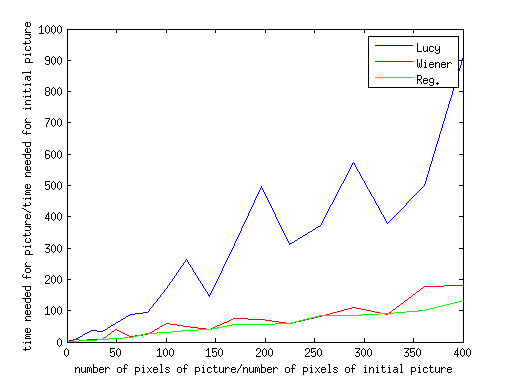
\includegraphics[{width= \textwidth}]{../Images/ComplexityRel.png}
\caption{The ratio ``time needed to compute the picture/ time needed to compute the smallest picture'' is the y axis and the x axis is the ratio ``number of pixels of the picture / number of pixels of the smallest picture''.}
\end{subfigure}~
\begin{subfigure}{0.4\textwidth}
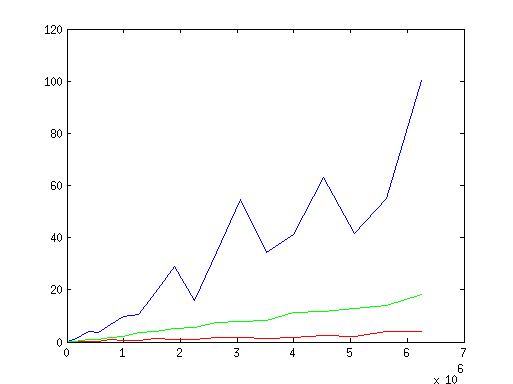
\includegraphics[{width= \textwidth}]{../Images/ComplexityAbs.png}
\caption{Time  needed to compute the picture on the y-axis, number of pixels of the picture on the x-axis.}
\end{subfigure}
\caption{Complexity of our different algorithms. The blue line is for \texttt{deconvLucy}, the red one for \texttt{deconvwnr} and the green one for \texttt{deconvreg}.}
\label{fig:Complexity}
\end{figure}



Let's now have a look at the complexity of our \texttt{robust\_angle\_estimator} method. Proceeding in the same way as for the deconvolution algorithms, we generate the plot shown in figure \ref{fig:ComplexityRadon}. The result are more surprising. Indeed, until a certain number of pixels, the relation between time and number of pixels seems linear. However, at around 100 times more pixels than with the starting picture, the time required starts to decline and then levels off at around 11 seconds. Either we computed something wrong, or matlab does some things strange. In all cases, there is here possibility for investigation.


\begin{figure}[h!]
\centering
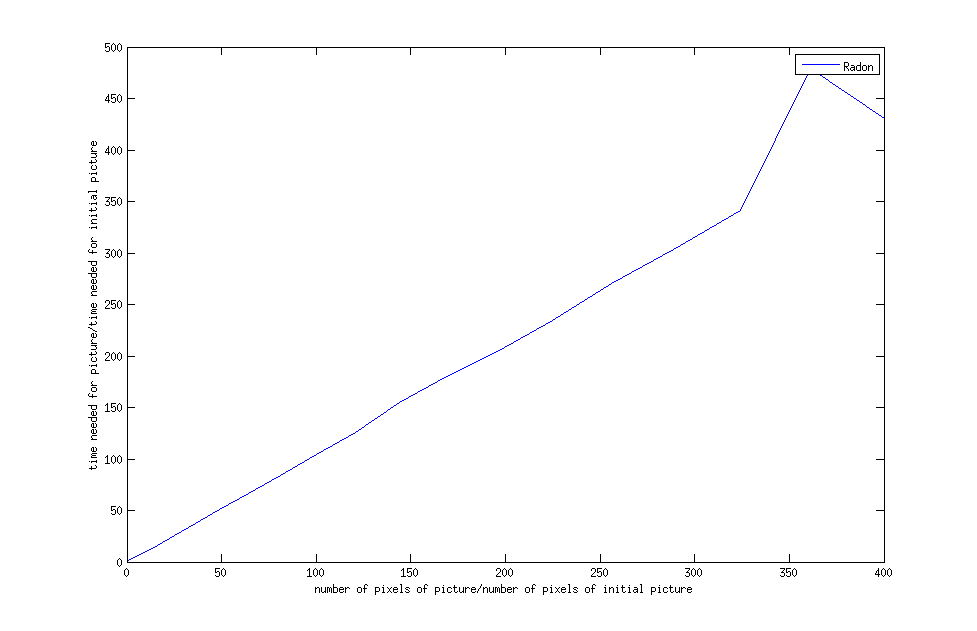
\includegraphics[scale=0.4]{../Images/ComplexityRadon.png}
\caption{Complexity of our \texttt{robust\_angle\_estimator} method}
\label{fig:ComplexityRadon}
\end{figure}






\end{document}
